
\section{单自由度非线性振动}
\subsection{微扰展开}
在非线性微扰 \(\epsilon f(x, \dot{x})\) 作用下，阻尼振动项为
\begin{equation*}
	G (x, \dot{x}, \ddot{x}) = \ddot{x} + 2 \zeta \omega_0 \dot{x} + \omega_0^2 x - \epsilon f(x, \dot{x})
\end{equation*}
其中无量纲常量\(\epsilon\)表征微扰阶数，阻尼项量级规定为 \(\zeta \sim \epsilon\).

方便起见，以下特征振动量\(x\)均不带量纲 (这总能通过重新定标实现)，上加点表示对时间\(t\)求导，固有频率\(\omega_0\) 具有 \(t^{-1}\) 的量纲.

引入\(T_n = \epsilon^n t\)表示不同尺度的时间变量，不同 \(T_n\) 之间相互独立，振动方程的解、关于时间的微分可展开为
\begin{equation*}
	x (t) = \sum_{n=0}^m \epsilon^n x_n (T_0, \dots, T_m),\quad
	\dfrac{\d}{\d t} = \sum_{n=0}^m \epsilon^n \dfrac{\partial}{\partial T_n} = \sum_{n=0}^m \epsilon^n D_n, \quad \dfrac{\d^2}{\d t^2} = \left( \sum_{n=0}^m \epsilon^n D_n \right)^2.
\end{equation*}
其中最高阶数  \(m\)视所需精度而定，\(D_n = \dfrac{\partial}{\partial T_n}\) 为偏微分算符，比如，展开到  \(m = 2\) 阶为
\begin{equation*}
	x (t) = x_0 (T_0, T_1, T_2) + \epsilon x_1 (T_0, T_1, T_2) + \epsilon^2 x_2 (T_0, T_1, T_2).
\end{equation*}
\begin{equation*}
	\dfrac{\d}{\d t} = D_0 + \epsilon D_1 + \epsilon^2 D_2, \quad \dfrac{\d^2}{\d t^2} = D_0^2 + 2 \epsilon D_0 D_1 + \epsilon^2 (D_1^2 + 2 D_0 D_2).
\end{equation*}

此时阻尼振动项展开为
\begin{equation*}
	G \left( x, \dot{x}, \ddot{x} \right) &= \left( D_0^2 x_0 + \omega_0^2 x_0 \right) + \epsilon \left( D_0^2 x_1 + \omega_0^2 x_1 + 2 D_0 D_1 x_0 - f \left( x_0, D_0 x_0 \right) + 2 \omega_0 \zeta D_0 x_0 \right) \\
	&\,+ \epsilon^2 \left[ D_0^2 x_2 + \omega_0^2 x_2 + 2 D_0 D_1 x_1 + \left( D_1^2 + 2 D_0 D_2 \right) x_0 - \left. \dfrac{\partial f}{\partial x} \right|_{\left( x_0, \dot{x}_0 \right)} x_1 - \left. \dfrac{\partial f}{\partial \dot{x}} \right|_{\left( x_0, \dot{x}_0 \right)} \dot{x}_1 + 2 \omega_0 \zeta \left( D_0 x_1 + D_1 x_0 \right) \right].
\end{equation*}

当然，在大多数问题中，展开到\(m = 1\)项即可得到大致准确的物理图像，以下问题也只精确至该阶，即
\begin{equation*}
	G (x, \dot{x}, \ddot{x}) = (D_0^2 x_0 + \omega_0^2 x_0) + \epsilon\left(D_0^2 x_1 + \omega_0^2 x_1 + 2 D_0 D_1 x_0 + 2 \omega_0 \zeta D_0 x_0 - f(x_0, D_0 x_0)\right).
\end{equation*}

\subsection{特殊频率处的振动}

\subsubsection{无外界驱动的自由振动}

代入\(G (x, \dot{x}, \ddot{x}) = 0\)，根据\(G\)的展开式，令各阶\(\epsilon\)的系数为零，得
\begin{equation*}
	D_0^2 x_0 + \omega_0^2 x_0 = 0,\quad D_0^2 x_1 + \omega_0^2 x_1 + 2 D_0 D_1 x_0 - f(x_0, D_0 x_0) + 2 \omega_0 \zeta D_0 x_0 = 0.
\end{equation*}

第一个方程解得
\begin{equation*}
	x_0 = a (T_1) \cos(\omega_0 T_0 + \theta (T_1)).
\end{equation*}
在无非线性项时\(a\)和\(\theta\)不随时间变化，进而与\(T_0\) 无关.

记\(\psi (T_0, T_1) = \omega_0 T_0 + \theta (T_1)\), 代入第二个方程得
\begin{equation*}
	D_0^2 x_1 + \omega_0^2 x_1 = 2 \omega_0 (D_1 a + \zeta a) \sin\psi + 2 \omega_0 a (D_1 \theta) \cos\psi + f(a \cos\psi, -\omega_0 a \sin\psi).
\end{equation*}

将\(f\)展开为傅里叶级数
\begin{equation*}
	f(a \cos\psi, -\omega_0 a \sin\psi) = \sum_{n=0}^\infty (c_n \cos(n\psi) + d_n \sin(n\psi)).
\end{equation*}
\begin{equation*}
	c_n = \dfrac{1}{(1 + \delta_{n0})\pi} \int_0^{2\pi} f(a \cos\psi', -\omega_0 a \sin\psi') \cos(n\psi') \,\d \psi', \quad d_n = \dfrac{1}{\pi} \int_0^{2\pi} f(a \cos\psi', -\omega_0 a \sin\psi') \sin(n\psi') \,\d \psi'.
\end{equation*}

为避免久期项 （即关于  \(x_1\) 的驱动力中会导致共振发散的  \(\cos\psi\) 和\(\sin\psi\) 项），要求
\begin{equation*}
	2 \omega_0 (D_1 a + \zeta a) + d_1 = 0,\quad
	2 \omega_0 a (D_1 \theta) + c_1 = 0.
\end{equation*}
其中
\begin{equation*}
	\Phi(a) = \dfrac{1}{2 \pi \omega_0^2} \int_0^{2\pi} f(a \cos\psi', -\omega_0 a \sin\psi') \sin\psi' \,\d \psi',
\end{equation*}
\begin{equation*}
	\Psi(a) = \dfrac{1}{2 \pi \omega_0^2} \int_0^{2\pi} f(a \cos\psi', -\omega_0 a \sin\psi') \cos\psi' \,\d \psi'.
\end{equation*}

转换成关于\(t\)的普通微分，得
\begin{equation*}
	\dot{a} = -\omega_0 \zeta a - \epsilon \omega_0 \Phi(a), \quad a \dot{\theta} = -\epsilon \omega_0 \Psi(a).
\end{equation*}

可见，\(\Phi\)给出了等效阻尼的非线性修正， \(\Psi\)给出了等效频率的非线性修正。稳恒态下，\(\dot{a} = 0,\,\dot{\theta} = 0\)，\(\theta_{\mathrm{s}}\) 任取，振幅满足
\begin{equation*}
	\zeta a_{\mathrm{s}} + \epsilon \Phi(a_{\mathrm{s}}) = 0, \quad \Psi(a_{\mathrm{s}}) = 0.
\end{equation*}

在稳态附近微扰，记  \(\xi = a - a_{\mathrm{s}}\), \(\eta = \theta - \theta_{\mathrm{s}}\)，保留至最低阶小量得
\begin{equation*}
	\dot{\xi} = -\left( \omega_0 \zeta + \epsilon \omega_0 \left. \dfrac{\partial \Phi}{\partial a} \right|_{a_{\mathrm{s}}} \right) \xi, \quad \dot{\eta} = -\dfrac{\epsilon \omega_0}{a_{\mathrm{s}}} \left. \dfrac{\partial \Psi}{\partial a} \right|_{a_{\mathrm{s}}} \xi.
\end{equation*}

若微扰收敛，则要求
\begin{equation*}
	\zeta + \epsilon \left. \dfrac{\partial \Phi}{\partial a} \right|_{a_{\mathrm{s}}} > 0.
\end{equation*}

\subsubsection{在固有频率附近驱动}

代入\(G (x, \dot{x}, \ddot{x}) = \epsilon \omega_0^2 B \cos(\omega t),\,\omega \approx \omega_0\)，记 \(\omega^2 = \omega_0^2 (1 + \epsilon \sigma)\)，为防止发散，量级上规定 \(B \sim 1\)，根据\(G\)的展开式，令各阶\(\epsilon\)的系数为零，得
\begin{equation*}
	D_0^2 x_0 + \omega^2 x_0 = 0,
\end{equation*}
\begin{equation*}
	D_0^2 x_1 + \omega^2 x_1 + 2 D_1 D_0 x_0 - f(x_0, D_0 x_0) + 2 \omega_0 \zeta D_0 x_0 - \omega_0^2 \sigma x_0 - \omega_0^2 B \cos(\omega t) = 0.
\end{equation*}

第一个方程解得
\begin{equation*}
	x_0 = a(T_1) \cos(\omega T_0 + \theta(T_1)).
\end{equation*}

记 \(\psi(T_0, T_1) = \omega T_0 + \theta(T_1)\)，代入第二个方程得
\begin{equation*}
	D_0^2 x_1 + \omega^2 x_1 = 2 \omega (D_1 a + \zeta a) \sin\psi + 2 \omega a (D_1 \theta) \cos\psi + f(a \cos\psi, -\omega a \sin\psi) + \omega_0^2 B \cos(\psi - \theta) - \omega_0^2 \sigma a \cos\psi.
\end{equation*}

同上，将\(f\)展开为傅里叶级数，为避免久期项得
\begin{equation*}
	2 \omega (D_1 a + \zeta a) + \omega_0^2 B \sin\theta + 2 \omega_0^2 \Phi(s, a) = 0,
\end{equation*}
\begin{equation*}
	2 \omega a (D_1 \theta) + \omega_0^2 B \cos\theta - \omega_0^2 \sigma a + 2 \omega_0^2 \Psi(s, a) = 0.
\end{equation*}
其中
\begin{equation*}
	\Phi(s, a) = \dfrac{1}{2 \pi \omega_0^2} \int_0^{2\pi} f(a \cos\psi', -\omega a \sin\psi') \sin\psi' \,\d \psi',
\end{equation*}
\begin{equation*}
	\Psi(s, a) = \dfrac{1}{2 \pi \omega_0^2} \int_0^{2\pi} f(a \cos\psi', -\omega a \sin\psi') \cos\psi' \,\d \psi'.
\end{equation*}

转换成关于\(t\)的普通微分，记\(s = \omega/\omega_0\)，并代入 \(\sigma = (s^2 - 1)/\epsilon\)，得
\begin{equation*}
	\dot{a} &= -\dfrac{\omega_0}{2 s} \left( 2 \zeta s a + \epsilon B \sin\theta + 2 \epsilon \Phi(s, a) \right)\\
	\dot{\theta} &= \dfrac{\omega_0}{2 s} \left( 1 - s^2 - \dfrac{\epsilon B}{a} \cos\theta - \dfrac{2 \epsilon}{a} \Psi(s, a) \right).
\end{equation*}

稳恒态下，\(\dot{a} = 0\)，\(\dot{\theta} = 0\)，得
\begin{equation*}
	B \sin\theta_{\mathrm{s}} &= -2 \zeta s a_{\mathrm{s}} - 2 \epsilon \Phi(s, a_{\mathrm{s}})\\
	B \cos\theta_{\mathrm{s}} &= \dfrac{a_{\mathrm{s}}}{\epsilon} (1 - s^2) - 2 \Psi(s, a_{\mathrm{s}}).
\end{equation*}
进而
\begin{equation*}
	\left( \Phi_s + \zeta s a_{\mathrm{s}} \right)^2 + \left( \Psi_s + \dfrac{a_{\mathrm{s}} (s^2 - 1)}{2 \epsilon} \right)^2 = \dfrac{B^2}{4},\quad
	\theta_{\mathrm{s}} = \arctan\left( \dfrac{2 (\zeta s a_{\mathrm{s}} + \epsilon \Phi_s)}{a_{\mathrm{s}} (s^2 - 1) + 2 \epsilon \Psi_s} \right).
\end{equation*}

在稳态附近微扰，记 \(\xi = a - a_{\mathrm{s}}\)，\(\eta = \theta - \theta_{\mathrm{s}}\)，保留至最低阶小量得
\begin{equation*}
	\dot{\xi} &= -\omega_0 \left( \zeta + \dfrac{\epsilon}{s} \left. \dfrac{\partial \Phi}{\partial a} \right|_s \right) \xi - \dfrac{\omega_0}{2 s} \left( a_{\mathrm{s}} (1 - s^2) - 2 \epsilon \Psi_s \right) \eta\\
	\dot{\eta} &= -\omega_0 \left( \zeta + \dfrac{\epsilon \Phi_s}{s a_{\mathrm{s}}} \right) \eta + \dfrac{\omega_0}{2 s a_{\mathrm{s}}} \left( (1 - s^2) - 2 \epsilon \left. \dfrac{\partial \Psi}{\partial a} \right|_s \right) \xi.
\end{equation*}

设扰动量随时间变化关系为 \(\xi, \eta \propto e^{\lambda \omega_0 t}\)，代入得
\begin{equation*}
	(\lambda + \zeta)^2 + 2 p (\lambda + \zeta) + q = 0 \implies \lambda = -\zeta - p \pm \sqrt{p^2 - q}
\end{equation*}
其中
\begin{equation*}
	p = \left. \dfrac{\epsilon}{2 s a_{\mathrm{s}}} \dfrac{\partial (a \Phi)}{\partial a} \right|_s,\quad
	q = \dfrac{\epsilon^2}{2 s^2 a_{\mathrm{s}}} \left. \dfrac{\partial}{\partial a} \left( \Phi^2 + \left( \Psi + \dfrac{a (s^2 - 1)}{2 \epsilon} \right)^2 \right) \right|_s.
\end{equation*}

对微扰收敛的 \((a_{\mathrm{s}}, \theta_{\mathrm{s}})\) 要求 \(\Re\lambda< 0\)，也即
\begin{equation*}
	p > -\zeta, \quad q > -\zeta^2 - 2 p \zeta.
\end{equation*}

一些特殊的非线性项例子如下：

\begin{example}
	Duffing系统，\(f(x, \dot{x}) = -\omega_0^2 x^3\).
	\begin{equation*}
		\Phi = 0, \quad \Psi = -\dfrac{3}{8} a^3.
	\end{equation*}

	稳恒态下
	\begin{equation*}
		(2 \zeta s)^2 + \left( s^2 - 1 - \dfrac{3}{4} \epsilon a_{\mathrm{s}}^2 \right)^2 = \dfrac{\epsilon^2 B^2}{a_{\mathrm{s}}^2}, \quad \theta_{\mathrm{s}} = \arctan\left( \dfrac{2 \zeta s}{s^2 - 1 - \dfrac{3}{4} \epsilon a_{\mathrm{s}}^2} \right).
	\end{equation*}
	\begin{equation*}
		p = 0, \quad q = \dfrac{1}{4 s^2} \left( s^2 - 1 - \dfrac{3}{4} \epsilon a_{\mathrm{s}}^2 \right) \left( s^2 - 1 - \dfrac{9}{4} \epsilon a_{\mathrm{s}}^2 \right).
	\end{equation*}

	稳定性条件给出
	\begin{equation*}
		\zeta > 0, \quad \epsilon^2 a_{\mathrm{s}}^4 - \dfrac{16}{9} (s^2 - 1) \epsilon a_{\mathrm{s}}^2 + \dfrac{16}{27} \left( (s^2 - 1)^2 + 4 \zeta^2 s^2 \right) > 0.
	\end{equation*}

	\begin{figure}[H]
		\centering
		\begin{subfigure}[b]{0.49\textwidth}
			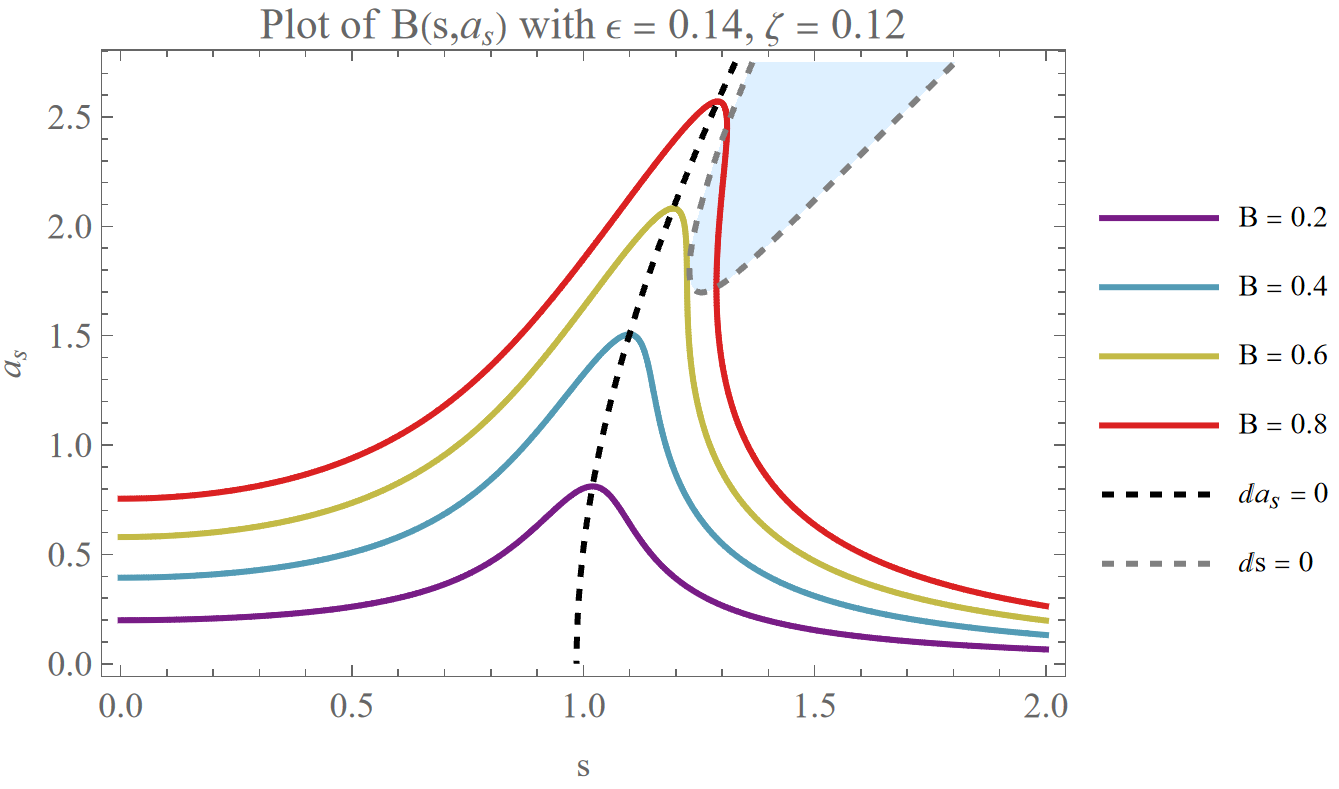
\includegraphics[width=\textwidth]{nonlinear_oscillation_fig/duffing_near_resonance_phase_portrait_epsilon_positive.png}
			\caption{\(\epsilon>0\)}
			\label{达芬系统固有频率附近驱动响应相图-epsilon>0}
		\end{subfigure}
		\hfill
		\begin{subfigure}[b]{0.49\textwidth}
			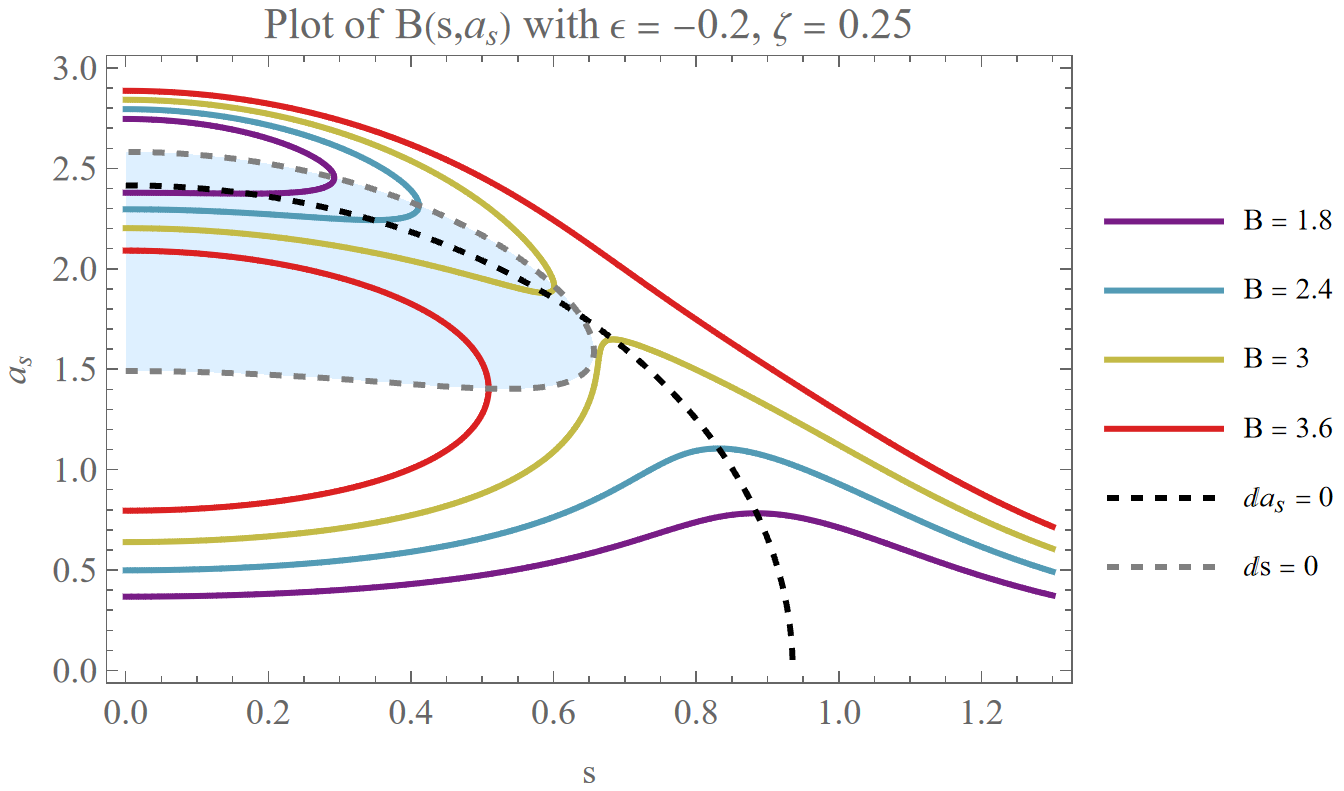
\includegraphics[width=\textwidth]{nonlinear_oscillation_fig/duffing_near_resonance_phase_portrait_epsilon_negative.png}
			\caption{\(\epsilon<0\)}
			\label{达芬系统固有频率附近驱动响应相图-epsilon<0}
		\end{subfigure}
		\caption{达芬系统固有频率附近驱动响应相图}
		\label{达芬系统固有频率附近驱动响应相图}
	\end{figure}

	相图如图\ref{达芬系统固有频率附近驱动响应相图}，不稳定区域用阴影标出，阴影的边界（\(\partial s/\partial a_{\mathrm{s}} = 0\)）为
	\begin{equation*}
		\epsilon a_{\mathrm{s}}^2 = \dfrac{8}{9} \left( s^2 - 1 \pm \dfrac{1}{2} \sqrt{(s^2 - 1)^2 - 12 \zeta^2 s^2} \right).
	\end{equation*}
	振幅 \(a_{\mathrm{s}}\) 取极值的线为（即 \(\partial a_{\mathrm{s}}/\partial s = 0\)）
	\begin{equation*}
		\epsilon a_{\mathrm{s}}^2 = \dfrac{4}{3} \left( 2 \zeta^2 + s^2 - 1 \right).
	\end{equation*}

	特别地，相图开始出现不稳定区域的临界振动量为
	\begin{equation*}
		&(s_c^2 - 1)^2 - 12 \zeta^2 s_c^2 = 0\quad \implies\quad s_c = \sqrt{1 + 3 \zeta^2} + \text{sgn}(\epsilon) \sqrt{3} \zeta.\\
		&a_{\mathrm{sc}}^2 = \dfrac{16 \sqrt{3}}{9} \dfrac{\zeta}{|\epsilon|} \left( \sqrt{1 + 3 \zeta^2} + \text{sgn}(\epsilon) \sqrt{3} \zeta \right),\\
		&B_{\mathrm{c}} = \dfrac{16 \sqrt{3 \sqrt{3}}}{9} \sqrt{\dfrac{\zeta^3}{|\epsilon|^3} \left( \sqrt{1 + 3 \zeta^2} + \text{sgn}(\epsilon) \sqrt{3} \zeta \right)^3}.
	\end{equation*}
\end{example}

\begin{example}
	自激系统，\(f(x, \dot{x}) = \omega_0 \dot{x} (1 - x^2)\).

	\begin{equation*}
		\Phi = -\dfrac{1}{2} s a \left( 1 - \dfrac{a^2}{4} \right), \quad \Psi = 0.
	\end{equation*}

	稳恒态下
	\begin{equation*}
		s^2 \left( 2 \zeta - \epsilon \left( 1 - \dfrac{a_{\mathrm{s}}^2}{4} \right) \right)^2 + (s^2 - 1)^2 = \dfrac{\epsilon^2 B^2}{a_{\mathrm{s}}^2}, \quad \theta_{\mathrm{s}} = \arctan\left( \dfrac{s \left( 2 \zeta - \epsilon \left( 1 - \dfrac{a_{\mathrm{s}}^2}{4} \right) \right)}{s^2 - 1} \right).
	\end{equation*}
	\begin{equation*}
		p = \dfrac{\epsilon}{4} (a_{\mathrm{s}}^2 - 2), \quad q = \dfrac{1}{4 s^2} \left( \epsilon^2 s^2 \left( 1 - \dfrac{a_{\mathrm{s}}^2}{4} \right) \left( 1 - \dfrac{3 a_{\mathrm{s}}^2}{4} \right) + (s^2 - 1)^2 \right).
	\end{equation*}

	稳定性条件给出
	\begin{equation*}
		a_{\mathrm{s}}^2 &> \text{max}\left[2 \left( 1 - \dfrac{2 \zeta}{\epsilon} \right),\quad\dfrac{8}{3} \left( 1 - \dfrac{2 \zeta}{\epsilon} \right) \left( 1 + \dfrac{1}{2} \sqrt{1 - 3 \left( \dfrac{s^2 - 1}{s (\epsilon - 2 \zeta)} \right)^2} \right)
			\right]\\
		a_{\mathrm{s}}^2 &< \dfrac{8}{3} \left( 1 - \dfrac{2 \zeta}{\epsilon} \right) \left( 1 - \dfrac{1}{2} \sqrt{1 - 3 \left( \dfrac{s^2 - 1}{s (\epsilon - 2 \zeta)} \right)^2} \right).
	\end{equation*}
\end{example}

\begin{example}
	干摩擦系统，\(f(x, \dot{x}) = -\omega_0^2 f_0 \text{sgn}(\dot{x}),\,f_0 > 0\).

	\begin{equation*}
		\Phi = \dfrac{2}{\pi} f_0, \quad \Psi = 0.
	\end{equation*}

	稳恒态下
	\begin{equation*}
		\left( \dfrac{4 \epsilon}{\pi a_{\mathrm{s}}} f_0 + 2 \zeta s \right)^2 + (s^2 - 1)^2 = \dfrac{\epsilon^2 B^2}{a_{\mathrm{s}}^2}, \quad \theta_{\mathrm{s}} = \arctan\left( \dfrac{2 \left( \zeta s + \dfrac{2 \epsilon}{\pi a_{\mathrm{s}}} f_0 \right)}{s^2 - 1} \right).
	\end{equation*}
	\begin{equation*}
		p = \dfrac{\epsilon f_0}{\pi s a_{\mathrm{s}}}, \quad q = \left( \dfrac{s^2 - 1}{2 s} \right)^2.
	\end{equation*}

	稳定性条件给出 \(\zeta > 0\).
\end{example}

\begin{example}
	湿摩擦系统，\(f(x, \dot{x}) = -\dfrac{\gamma \dot{x} |\dot{x}|}{\epsilon},\,\gamma > 0\).

	\begin{equation*}
		\Phi = \dfrac{4 \gamma}{3 \pi \epsilon} s^2 a_{\mathrm{s}}^2, \quad \Psi = 0.
	\end{equation*}

	稳恒态下
	\begin{equation*}
		s^2 \left( \dfrac{8 \gamma}{3 \pi} s a_{\mathrm{s}} + 2 \zeta \right)^2 + (s^2 - 1)^2 = \dfrac{\epsilon^2 B^2}{a_{\mathrm{s}}^2}, \quad \theta_{\mathrm{s}} = \arctan\left( \dfrac{s \left( \dfrac{8 \gamma}{3 \pi} s a_{\mathrm{s}} + 2 \zeta \right)}{s^2 - 1} \right).
	\end{equation*}
	\begin{equation*}
		p = \left. \dfrac{\epsilon}{2 s a_{\mathrm{s}}} \dfrac{\partial (a \Phi)}{\partial a} \right|_s = \dfrac{2 \gamma s a_{\mathrm{s}}}{\pi},\quad
		q = \dfrac{\epsilon^2}{2 s^2 a_{\mathrm{s}}} \left. \dfrac{\partial}{\partial a} \left( \Phi^2 + \left( \Psi + \dfrac{a (s^2 - 1)}{2 \epsilon} \right)^2 \right) \right|_s = \left( \dfrac{s^2 - 1}{2 s} \right)^2 + \dfrac{32 \gamma^2}{9 \pi^2} s^2 a_{\mathrm{s}}^2.
	\end{equation*}
\end{example}

\subsubsection{在远离固有频率处驱动}

代入\(G (x, \dot{x}, \ddot{x}) = \omega_0^2 F \cos(\omega t),\,|\omega - \omega_0|/\omega_0\sim 1\)，此时，\(F\)对\(x\)的影响在 \(x_0\) 阶即可不发散地体现，因此在量级上 \(F \sim 1\)，各阶振动方程为
\begin{equation*}
	D_0^2 x_0 + \omega_0^2 x_0 - F \cos(\omega t) = 0,\quad
	D_0^2 x_1 + \omega_0^2 x_1 + 2 D_1 D_0 x_0 - f(x_0, D_0 x_0) + 2 \omega_0 \zeta D_0 x_0 = 0.
\end{equation*}

第一个方程解得
\begin{equation*}
	x_0 = A \cos(\omega T_0) + a(T_1) \cos(\omega_0 T_0 + \theta(T_1))
\end{equation*}
其中\(A = F \left( 1 - \omega^2/\omega_0^2 \right)^{-1}\).

记
\begin{equation*}
	\Phi(T_0, T_1) = \omega T_0,\quad \psi(T_0, T_1) = \omega_0 T_0 + \theta(T_1)\quad\implies\quad x_0 = A \cos\Phi + a \cos\psi
\end{equation*}
其中，由于\(\omega\)与\(\omega_0\)某一倍数之差可能含\(\epsilon\)的线性项，因此\(\Phi\)可能含有\(T_1\)项。

代入第二个方程得
\begin{equation*}
	\begin{aligned}
		D_0^2 x_1 + \omega_0^2 x_1 & = 2 \omega_0 \left( D_1 a + \omega_0 \zeta a \right) \sin\psi + 2 \omega_0 a (D_1 \theta) \cos\psi + 2 \omega A (D_1 \Phi) \cos\Phi + 2 \omega \omega_0 \zeta A \sin\Phi \\
		                           & \quad + f\left( A \cos\Phi + a \cos\psi, -\omega A \sin\Phi - \omega_0 a \sin\psi \right).
	\end{aligned}
\end{equation*}

对于一般的\(f(x, \dot{x})\)，上式右侧的久期项与无驱动力时相同，处理方法如前.而对于较为特殊的\(f(x, \dot{x})\)（比如恰含 \(x\)或 \(\dot{x}\) 的相应有理数幂次），则当\(\omega\) 接近于 \(\omega_0\) 的某个有理数倍时，才可能出现新的 久期项.

在Duffing系统中，\(f(x, \dot{x}) = -\omega_0^2 x^3\)，也即振动方程为
\begin{equation*}
	\ddot{x} + 2 \zeta \omega_0 \dot{x} + \omega_0^2 x (1 + \epsilon x^2) = F_0 \cos(\omega t)
\end{equation*}
代入 \(x_1\) 的振动方程得
\begin{equation*}
	D_0^2 x_1 &+ \omega_0^2 x_1 = 2 \omega_0 \left( D_1 a + \omega_0 \zeta a \right) \sin\psi + 2 \omega_0 a \left( D_1 \theta - \dfrac{3}{8} \omega_0 \left( a^2 + 2 A^2 \right) \right) \cos\psi \\
	&\,+ 2 \omega \omega_0 \zeta A \sin\Phi + 2 \omega A \left( D_1 \Phi - \dfrac{3 \omega_0^2}{8 \omega} \left( 2 a^2 + A^2 \right) \right) \cos\Phi \\
	&\,- \dfrac{1}{4} \omega_0^2 \left( a^3 \cos \left( 3\psi \right) + A^3 \cos \left( 3\Phi \right) \right) - \dfrac{3}{4} \omega_0^2 aA \left( a \left( \cos \left( \Phi + 2\psi \right) + \cos \left( \Phi - 2\psi \right) \right) + A \left( \cos \left( \psi + 2\Phi \right) + \cos \left( \psi - 2\Phi \right) \right) \right)\\
	&\qquad\approx 2 \omega_0 \left( D_1 a + \omega_0 \zeta a \right) \sin\psi + 2 \omega_0 a \left( D_1 \theta - \dfrac{3}{8} \omega_0 \left( a^2 + 2 A^2 \right) \right) \cos\psi - \dfrac{1}{4} \omega_0^2 A^3 \cos \left( 3\Phi \right) - \dfrac{3}{4} \omega_0^2 a^2 A \cos \left( \Phi - 2\psi \right).
\end{equation*}
最后一步仅保留右侧可能含\(\psi\)的正余弦的项，并用到\(|\Phi - \psi| \sim \psi.\)

可见，当 \(\Phi \approx \psi/3\) 或 \(\Phi \approx 3\psi\) 时，可能出现额外的久期项.

【情况1】超谐波共振，\(\omega \approx \omega_0/3\)

记 \(3\omega = \omega_0 (1 + \epsilon \sigma)\)，即 \(3\Phi = \psi - \gamma\)，\(\gamma = \theta - \sigma \omega_0 T_1\)，代入得（仅保留久期项）
\begin{equation*}
	D_0^2 x_1 + \omega_0^2 x_1 = 2 \omega_0 \left( D_1 a + \omega_0 \zeta a - \dfrac{\omega_0}{8} A^3 \sin\gamma \right) \sin\psi+ 2 \omega_0 a \left( D_1 \theta - \dfrac{3}{8} \omega_0 (a^2 + 2 A^2) - \dfrac{1}{8} \omega_0 \dfrac{A^3}{a} \cos\gamma \right) \cos\psi.
\end{equation*}
为避免久期项，得（用到 \(D_1 \gamma = D_1 \theta - \sigma \omega_0\)）
\begin{equation*}
	\dot{a} = \omega_0 \epsilon \left( -\zeta a + \dfrac{1}{8} A^3 \sin\gamma \right),\quad
	\dot{\gamma} = \omega_0 \epsilon \left( -\sigma + \dfrac{3}{8} (a^2 + 2 A^2) + \dfrac{1}{8} \dfrac{A^3}{a} \cos\gamma \right).
\end{equation*}

稳态下 \(\dot{a} = 0\)，\(\dot{\gamma} = 0\)，对应
\begin{equation*}
	A^3 \sin\gamma_{\mathrm{s}} = 8 \zeta a_{\mathrm{s}},\quad
	A^3 \cos\gamma_{\mathrm{s}} = \left( 8\sigma - 3(a_{\mathrm{s}}^2 + 2A^2) \right) a_{\mathrm{s}}.
\end{equation*}
也即
\begin{equation*}
	\left( 8\zeta a_{\mathrm{s}} \right)^2 + \left( 8\sigma - 3(a_{\mathrm{s}}^2 + 2A^2) \right)^2 a_{\mathrm{s}}^2 = A^6, \quad \gamma_{\mathrm{s}} = \arctan\left( \dfrac{8 \zeta a_{\mathrm{s}}}{8\sigma - 3(a_{\mathrm{s}}^2 + 2A^2)} \right).
\end{equation*}
记 \(s =\omega/\omega_0\)，代入 \(\sigma = (3s - 1)/\epsilon,\,A = F (1 - s^2)^{-1}\)，则上式等价为
\begin{equation*}
	\zeta^2 + \left( \dfrac{3s - 1}{\epsilon} - \dfrac{3}{8} a_{\mathrm{s}}^2 - \dfrac{3}{4} \dfrac{F^2}{(1 - s^2)^2} \right)^2 = \dfrac{F^6}{64 a_{\mathrm{s}}^2(1 - s^2)^6}.
\end{equation*}
三次方程至少有一个实根，因此 \(a_{\mathrm{s}}\) 必有实数解，即总可以形成超谐波共振.

此时
\begin{equation*}
	\psi = \omega_0 T_0 + \theta = \omega_0 t + \gamma_{\mathrm{s}} + \sigma \omega_0 \epsilon t = 3\omega t + \gamma_{\mathrm{s}}
\end{equation*}
因此\(x\)的振动主要由 \(\omega\) 和 \(3\omega\)的频率构成.
\begin{figure}[H]
	\centering
	\begin{subfigure}[b]{0.49\textwidth}
		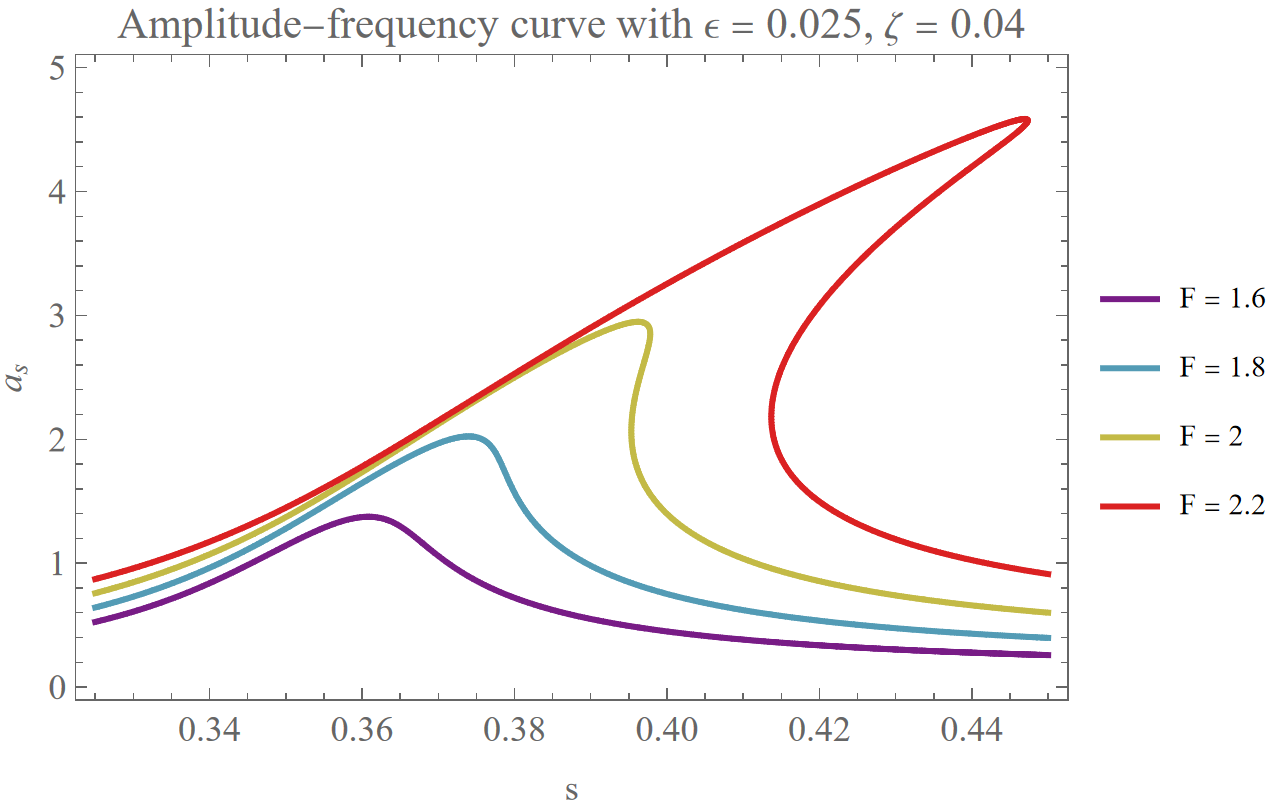
\includegraphics[width=\textwidth]{nonlinear_oscillation_fig/duffing_superharmonic_response_epsilon_positive.png}
		\caption{\(\epsilon>0\)}
		\label{达芬系统超谐波共振幅频响应图-epsilon>0}
	\end{subfigure}
	\hfill
	\begin{subfigure}[b]{0.49\textwidth}
		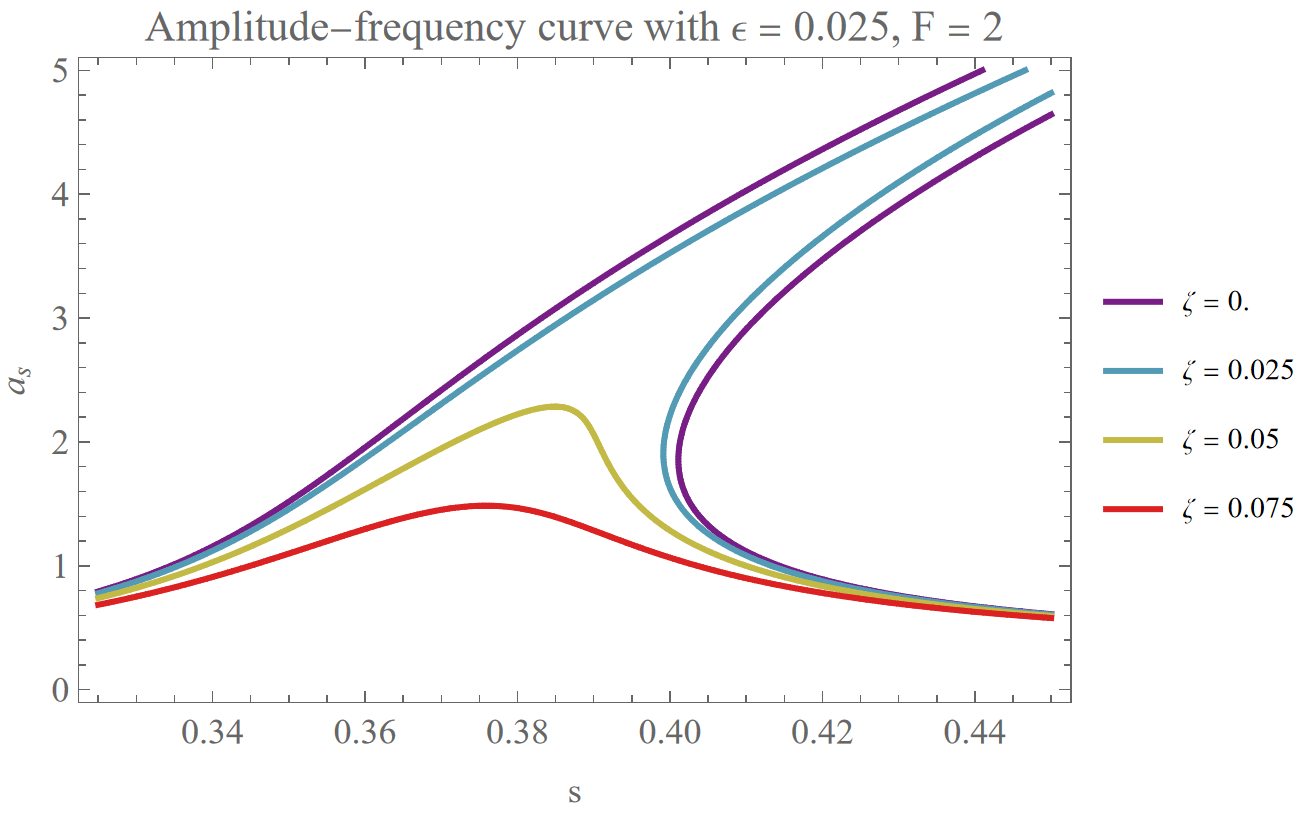
\includegraphics[width=\textwidth]{nonlinear_oscillation_fig/duffing_superharmonic_response_epsilon_negative.png}
		\caption{\(\epsilon<0\)}
		\label{达芬系统超谐波共振幅频响应图-epsilon<0}
	\end{subfigure}

	\caption{达芬系统超谐波共振幅频响应图}
	\label{达芬系统超谐波共振幅频响应图}
\end{figure}

【情况2】亚谐波共振，\(\omega \approx 3\omega_0\)

记 \(\omega = \omega_0 (3 + \epsilon \sigma)\)，即 \(\Phi = 3\psi - \gamma,\,\gamma = 3\theta - \sigma \omega_0 T_1\)，代入得（仅保留久期项）
\begin{equation*}
	D_0^2 x_1 + \omega_0^2 x_1 &= 2 \omega_0 \left( D_1 a + \omega_0 \zeta a - \dfrac{3 \omega_0}{8} a^2 A \sin\gamma \right) \sin\psi \\
	&\quad + 2 \omega_0 a \left( D_1 \theta - \dfrac{3}{8} \omega_0 (a^2 + 2A^2 + aA \cos\gamma) \right) \cos\psi.
\end{equation*}
为避免久期项，得（用到 \(D_1 \gamma = 3D_1 \theta - \sigma \omega_0\)）
\begin{equation*}
	\dot{a} = -\omega_0 \zeta a + \dfrac{3 \omega_0 a^2 A}{8} \sin\gamma,\quad \dot{\gamma} = \dfrac{9 \omega_0}{8} (a^2 + 2A^2 + aA \cos\gamma) - \omega_0 \sigma.
\end{equation*}
稳态下 \(\dot{a} = 0\)，\(\dot{\gamma} = 0\)，对应
\begin{equation*}
	A a_{\mathrm{s}} \sin\gamma_{\mathrm{s}} = \dfrac{8\zeta}{3},\quad A a_{\mathrm{s}} \cos\gamma_{\mathrm{s}} = \dfrac{8\sigma}{9} - a_{\mathrm{s}}^2 - 2A^2.
\end{equation*}
也即
\begin{equation*}
	\gamma_{\mathrm{s}} = \arctan\left( \dfrac{24\zeta}{8\sigma - 9(a_{\mathrm{s}}^2 + 2A^2)} \right), \quad a_{\mathrm{s}}^2 = p \pm \sqrt{p^2 - q}.
\end{equation*}
其中
\begin{equation*}
	s &= \frac{\omega}{\omega_0},\quad\sigma =\frac{s - 3}{\epsilon},\quad A =\frac{F}{1-s^2}\\
	p &= \dfrac{8}{9} \left( \sigma - \dfrac{27}{16} A^2 \right) = \dfrac{8}{9} \left( \dfrac{s - 3}{\epsilon} - \dfrac{27}{16} \dfrac{F^2}{(1 - s^2)^2} \right)\\
	q &= \dfrac{64}{81} \left( \dfrac{9\zeta^2}{\epsilon^2} + \left( \sigma - \dfrac{9A^2}{4} \right)^2 \right) = \dfrac{64}{81} \left( \dfrac{9\zeta^2}{\epsilon^2} + \left( \dfrac{s - 3}{\epsilon} - \dfrac{9}{4} \dfrac{F^2}{(1 - s^2)^2} \right)^2 \right).
\end{equation*}

稳定时，\(a_{\mathrm{s}}\) 存在实数解，故要求 \(p > 0\)，\(p^2 \geq q\) 即
\begin{equation*}
	\dfrac{27}{16} F^2 - (1 - s^2)^2 \dfrac{s - 3}{\epsilon} < 0,\quad
	\dfrac{63}{32} F^4 - (1 - s^2)^2 \dfrac{s - 3}{\epsilon} F^2 + 8 (1 - s^2)^4 \dfrac{\zeta^2}{\epsilon^2} \leq 0.
\end{equation*}
进而给出能够发生亚谐波共振的区域如图(\(A,\,\sigma\)与\(F,\,s\)的换算关系见上)，其中区域边界的函数关系为
\begin{equation*}
	F^2 = \dfrac{16}{63} (1 - s^2)^2 \left( \dfrac{s - 3}{\epsilon} \pm \sqrt{\left( \dfrac{s - 3}{\epsilon} \right)^2 - \dfrac{63\zeta^2}{\epsilon^2}} \right).
\end{equation*}

此时
\begin{equation*}
	\psi = \omega_0 T_0 + \theta = \omega_0 t + \frac{\gamma_{\mathrm{s}} + \sigma \omega_0 \epsilon t}{3}= \frac{\omega t + \gamma_{\mathrm{s}}}{3}
\end{equation*}
因此\(x\)的振动主要由 \(\omega\) 和 \(\omega/3\) 的频率构成.
\begin{figure}[H]
	\centering
	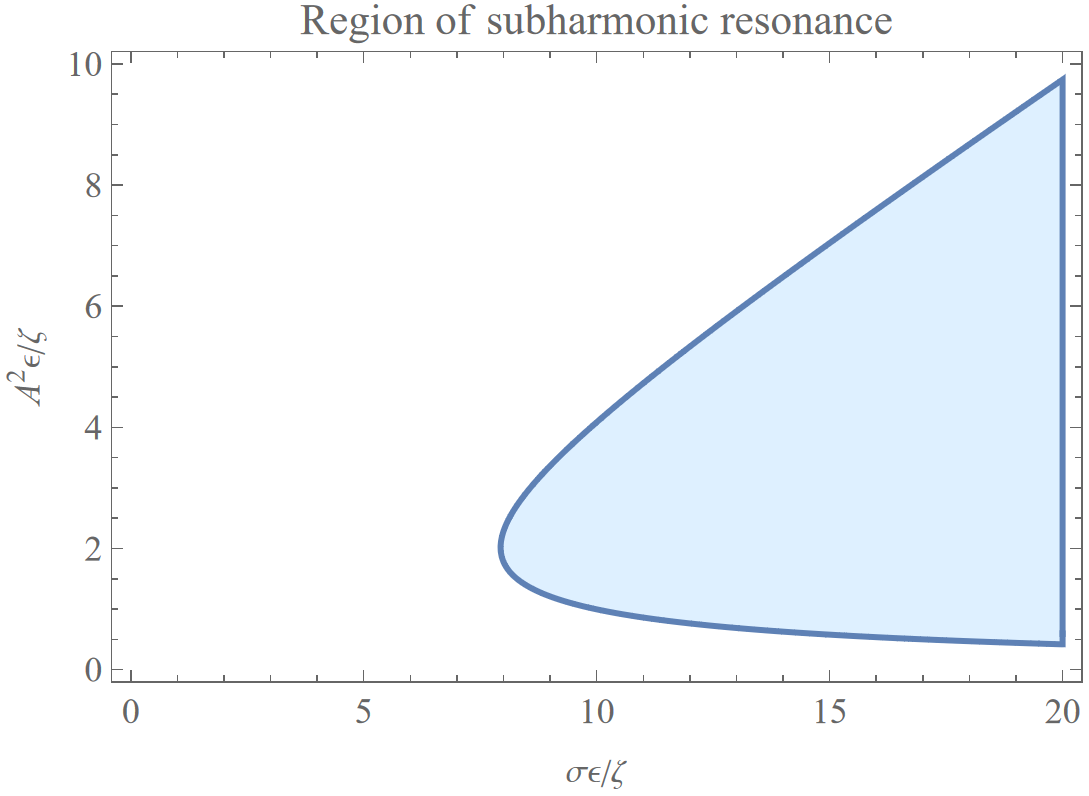
\includegraphics[width=0.4\textwidth]{nonlinear_oscillation_fig/duffing_system_subharmonic_resonance_response_plot.png}
	\caption{达芬系统亚谐波共振响应图}
	\label{达芬系统亚谐波共振响应图}
\end{figure}
